% Options for packages loaded elsewhere
\PassOptionsToPackage{unicode}{hyperref}
\PassOptionsToPackage{hyphens}{url}
\PassOptionsToPackage{dvipsnames,svgnames,x11names}{xcolor}
%
\documentclass[
  letterpaper,
  DIV=11,
  numbers=noendperiod]{scrartcl}

\usepackage{amsmath,amssymb}
\usepackage{iftex}
\ifPDFTeX
  \usepackage[T1]{fontenc}
  \usepackage[utf8]{inputenc}
  \usepackage{textcomp} % provide euro and other symbols
\else % if luatex or xetex
  \usepackage{unicode-math}
  \defaultfontfeatures{Scale=MatchLowercase}
  \defaultfontfeatures[\rmfamily]{Ligatures=TeX,Scale=1}
\fi
\usepackage{lmodern}
\ifPDFTeX\else  
    % xetex/luatex font selection
\fi
% Use upquote if available, for straight quotes in verbatim environments
\IfFileExists{upquote.sty}{\usepackage{upquote}}{}
\IfFileExists{microtype.sty}{% use microtype if available
  \usepackage[]{microtype}
  \UseMicrotypeSet[protrusion]{basicmath} % disable protrusion for tt fonts
}{}
\makeatletter
\@ifundefined{KOMAClassName}{% if non-KOMA class
  \IfFileExists{parskip.sty}{%
    \usepackage{parskip}
  }{% else
    \setlength{\parindent}{0pt}
    \setlength{\parskip}{6pt plus 2pt minus 1pt}}
}{% if KOMA class
  \KOMAoptions{parskip=half}}
\makeatother
\usepackage{xcolor}
\setlength{\emergencystretch}{3em} % prevent overfull lines
\setcounter{secnumdepth}{-\maxdimen} % remove section numbering
% Make \paragraph and \subparagraph free-standing
\makeatletter
\ifx\paragraph\undefined\else
  \let\oldparagraph\paragraph
  \renewcommand{\paragraph}{
    \@ifstar
      \xxxParagraphStar
      \xxxParagraphNoStar
  }
  \newcommand{\xxxParagraphStar}[1]{\oldparagraph*{#1}\mbox{}}
  \newcommand{\xxxParagraphNoStar}[1]{\oldparagraph{#1}\mbox{}}
\fi
\ifx\subparagraph\undefined\else
  \let\oldsubparagraph\subparagraph
  \renewcommand{\subparagraph}{
    \@ifstar
      \xxxSubParagraphStar
      \xxxSubParagraphNoStar
  }
  \newcommand{\xxxSubParagraphStar}[1]{\oldsubparagraph*{#1}\mbox{}}
  \newcommand{\xxxSubParagraphNoStar}[1]{\oldsubparagraph{#1}\mbox{}}
\fi
\makeatother


\providecommand{\tightlist}{%
  \setlength{\itemsep}{0pt}\setlength{\parskip}{0pt}}\usepackage{longtable,booktabs,array}
\usepackage{calc} % for calculating minipage widths
% Correct order of tables after \paragraph or \subparagraph
\usepackage{etoolbox}
\makeatletter
\patchcmd\longtable{\par}{\if@noskipsec\mbox{}\fi\par}{}{}
\makeatother
% Allow footnotes in longtable head/foot
\IfFileExists{footnotehyper.sty}{\usepackage{footnotehyper}}{\usepackage{footnote}}
\makesavenoteenv{longtable}
\usepackage{graphicx}
\makeatletter
\def\maxwidth{\ifdim\Gin@nat@width>\linewidth\linewidth\else\Gin@nat@width\fi}
\def\maxheight{\ifdim\Gin@nat@height>\textheight\textheight\else\Gin@nat@height\fi}
\makeatother
% Scale images if necessary, so that they will not overflow the page
% margins by default, and it is still possible to overwrite the defaults
% using explicit options in \includegraphics[width, height, ...]{}
\setkeys{Gin}{width=\maxwidth,height=\maxheight,keepaspectratio}
% Set default figure placement to htbp
\makeatletter
\def\fps@figure{htbp}
\makeatother

\KOMAoption{captions}{tableheading}
\makeatletter
\@ifpackageloaded{tcolorbox}{}{\usepackage[skins,breakable]{tcolorbox}}
\@ifpackageloaded{fontawesome5}{}{\usepackage{fontawesome5}}
\definecolor{quarto-callout-color}{HTML}{909090}
\definecolor{quarto-callout-note-color}{HTML}{0758E5}
\definecolor{quarto-callout-important-color}{HTML}{CC1914}
\definecolor{quarto-callout-warning-color}{HTML}{EB9113}
\definecolor{quarto-callout-tip-color}{HTML}{00A047}
\definecolor{quarto-callout-caution-color}{HTML}{FC5300}
\definecolor{quarto-callout-color-frame}{HTML}{acacac}
\definecolor{quarto-callout-note-color-frame}{HTML}{4582ec}
\definecolor{quarto-callout-important-color-frame}{HTML}{d9534f}
\definecolor{quarto-callout-warning-color-frame}{HTML}{f0ad4e}
\definecolor{quarto-callout-tip-color-frame}{HTML}{02b875}
\definecolor{quarto-callout-caution-color-frame}{HTML}{fd7e14}
\makeatother
\makeatletter
\@ifpackageloaded{caption}{}{\usepackage{caption}}
\AtBeginDocument{%
\ifdefined\contentsname
  \renewcommand*\contentsname{Table of contents}
\else
  \newcommand\contentsname{Table of contents}
\fi
\ifdefined\listfigurename
  \renewcommand*\listfigurename{List of Figures}
\else
  \newcommand\listfigurename{List of Figures}
\fi
\ifdefined\listtablename
  \renewcommand*\listtablename{List of Tables}
\else
  \newcommand\listtablename{List of Tables}
\fi
\ifdefined\figurename
  \renewcommand*\figurename{Figure}
\else
  \newcommand\figurename{Figure}
\fi
\ifdefined\tablename
  \renewcommand*\tablename{Table}
\else
  \newcommand\tablename{Table}
\fi
}
\@ifpackageloaded{float}{}{\usepackage{float}}
\floatstyle{ruled}
\@ifundefined{c@chapter}{\newfloat{codelisting}{h}{lop}}{\newfloat{codelisting}{h}{lop}[chapter]}
\floatname{codelisting}{Listing}
\newcommand*\listoflistings{\listof{codelisting}{List of Listings}}
\makeatother
\makeatletter
\makeatother
\makeatletter
\@ifpackageloaded{caption}{}{\usepackage{caption}}
\@ifpackageloaded{subcaption}{}{\usepackage{subcaption}}
\makeatother

\ifLuaTeX
  \usepackage{selnolig}  % disable illegal ligatures
\fi
\usepackage{bookmark}

\IfFileExists{xurl.sty}{\usepackage{xurl}}{} % add URL line breaks if available
\urlstyle{same} % disable monospaced font for URLs
\hypersetup{
  pdftitle={Calculus I Notes},
  colorlinks=true,
  linkcolor={blue},
  filecolor={Maroon},
  citecolor={Blue},
  urlcolor={Blue},
  pdfcreator={LaTeX via pandoc}}


\title{Calculus I Notes}
\author{Ross Dunne}
\date{}

\begin{document}
\maketitle


\subsection{Thomas Calculus Ch 3.
Notes}\label{thomas-calculus-ch-3.-notes}

\subsubsection{Definitions}\label{definitions}

\begin{tcolorbox}[enhanced jigsaw, left=2mm, colbacktitle=quarto-callout-note-color!10!white, coltitle=black, arc=.35mm, toptitle=1mm, opacityback=0, colback=white, colframe=quarto-callout-note-color-frame, breakable, bottomrule=.15mm, bottomtitle=1mm, opacitybacktitle=0.6, titlerule=0mm, leftrule=.75mm, toprule=.15mm, title=\textcolor{quarto-callout-note-color}{\faInfo}\hspace{0.5em}{Definition 1: Slope}, rightrule=.15mm]

The \textbf{slope} of the curve \(y = f(x)\) at the point
\(P(x_0, f(x_0))\) is the number

\[
\lim_{h \to 0} \frac{f(x_0 + h) - f(x_0)}{h} \quad \text{(provided the limit exists).}
\]

The \textbf{tangent line} to the curve at \(P\) is the line through
\(P\) with this slope.

\end{tcolorbox}

\begin{tcolorbox}[enhanced jigsaw, left=2mm, colbacktitle=quarto-callout-note-color!10!white, coltitle=black, arc=.35mm, toptitle=1mm, opacityback=0, colback=white, colframe=quarto-callout-note-color-frame, breakable, bottomrule=.15mm, bottomtitle=1mm, opacitybacktitle=0.6, titlerule=0mm, leftrule=.75mm, toprule=.15mm, title=\textcolor{quarto-callout-note-color}{\faInfo}\hspace{0.5em}{Definition 2: Derivative}, rightrule=.15mm]

The \textbf{derivative} of a function \(f\) at a point \(x_0\), denoted
\(f'(x_0)\), is \[
f'(x_0) = \lim_{h \to 0} \frac{f(x_0 + h) - f(x_0)}{h} \quad \text{(provided the limit exists).}
\]

\end{tcolorbox}

\begin{tcolorbox}[enhanced jigsaw, left=2mm, colbacktitle=quarto-callout-note-color!10!white, coltitle=black, arc=.35mm, toptitle=1mm, opacityback=0, colback=white, colframe=quarto-callout-note-color-frame, breakable, bottomrule=.15mm, bottomtitle=1mm, opacitybacktitle=0.6, titlerule=0mm, leftrule=.75mm, toprule=.15mm, title=\textcolor{quarto-callout-note-color}{\faInfo}\hspace{0.5em}{Definition 3: Alternative Derivative}, rightrule=.15mm]

\[
f'(x_0) = \lim_{h \to 0} \frac{f(z) - f(x)}{z-x} \quad \text{(provided the limit exists).}
\]

\end{tcolorbox}

\begin{tcolorbox}[enhanced jigsaw, left=2mm, colbacktitle=quarto-callout-note-color!10!white, coltitle=black, arc=.35mm, toptitle=1mm, opacityback=0, colback=white, colframe=quarto-callout-note-color-frame, breakable, bottomrule=.15mm, bottomtitle=1mm, opacitybacktitle=0.6, titlerule=0mm, leftrule=.75mm, toprule=.15mm, title=\textcolor{quarto-callout-note-color}{\faInfo}\hspace{0.5em}{Definition 4: Theorem 1}, rightrule=.15mm]

\textbf{Differentiable Implies Continuous} If \(f\) has a derivative at
\(x = c\), then \(f\) is continuous at \(x = c\).

\end{tcolorbox}

\begin{tcolorbox}[enhanced jigsaw, left=2mm, colbacktitle=quarto-callout-note-color!10!white, coltitle=black, arc=.35mm, toptitle=1mm, opacityback=0, colback=white, colframe=quarto-callout-note-color-frame, breakable, bottomrule=.15mm, bottomtitle=1mm, opacitybacktitle=0.6, titlerule=0mm, leftrule=.75mm, toprule=.15mm, title=\textcolor{quarto-callout-note-color}{\faInfo}\hspace{0.5em}{Definition 5: Derivative of a Constant Function}, rightrule=.15mm]

If \(f\) has the constant value \(f (x)= c\), then \[
\frac{df}{dx} = \frac{d}{dx}(c) = 0.
\]

\end{tcolorbox}

\begin{tcolorbox}[enhanced jigsaw, left=2mm, colbacktitle=quarto-callout-note-color!10!white, coltitle=black, arc=.35mm, toptitle=1mm, opacityback=0, colback=white, colframe=quarto-callout-note-color-frame, breakable, bottomrule=.15mm, bottomtitle=1mm, opacitybacktitle=0.6, titlerule=0mm, leftrule=.75mm, toprule=.15mm, title=\textcolor{quarto-callout-note-color}{\faInfo}\hspace{0.5em}{Definition 6: Derivative of a positive integer power}, rightrule=.15mm]

If \(n\) is a positive integer then \[
\frac{dx^n}{dx} = nx^{n-1}.
\]

\end{tcolorbox}

\begin{tcolorbox}[enhanced jigsaw, left=2mm, colbacktitle=quarto-callout-note-color!10!white, coltitle=black, arc=.35mm, toptitle=1mm, opacityback=0, colback=white, colframe=quarto-callout-note-color-frame, breakable, bottomrule=.15mm, bottomtitle=1mm, opacitybacktitle=0.6, titlerule=0mm, leftrule=.75mm, toprule=.15mm, title=\textcolor{quarto-callout-note-color}{\faInfo}\hspace{0.5em}{Definition 7: Derivative constant multiple rule}, rightrule=.15mm]

If \(u\) is a differentiable function of \(x\), and \(c\) is a constant,
then \[
\frac{d}{dx}(cu) = c\frac{du}{dx}
\]

\end{tcolorbox}

\begin{tcolorbox}[enhanced jigsaw, left=2mm, colbacktitle=quarto-callout-note-color!10!white, coltitle=black, arc=.35mm, toptitle=1mm, opacityback=0, colback=white, colframe=quarto-callout-note-color-frame, breakable, bottomrule=.15mm, bottomtitle=1mm, opacitybacktitle=0.6, titlerule=0mm, leftrule=.75mm, toprule=.15mm, title=\textcolor{quarto-callout-note-color}{\faInfo}\hspace{0.5em}{Definition 8: Derivative sum rule}, rightrule=.15mm]

If \(u\) and \(v\) are differentiable functions of \(x\), then their sum
\(u + v\) is differentiable at every point where \(u\) and \(v\) are
both differentiable. At such points: \[
\frac{d}{dx}(u + v) = \frac{du}{dx} + \frac{dv}{dx}
\]

\end{tcolorbox}

\begin{tcolorbox}[enhanced jigsaw, left=2mm, colbacktitle=quarto-callout-note-color!10!white, coltitle=black, arc=.35mm, toptitle=1mm, opacityback=0, colback=white, colframe=quarto-callout-note-color-frame, breakable, bottomrule=.15mm, bottomtitle=1mm, opacitybacktitle=0.6, titlerule=0mm, leftrule=.75mm, toprule=.15mm, title=\textcolor{quarto-callout-note-color}{\faInfo}\hspace{0.5em}{Definition 9: Derivative of e}, rightrule=.15mm]

\[
\frac{d}{dx}(e^x) = e^x
\]

\end{tcolorbox}

\begin{tcolorbox}[enhanced jigsaw, left=2mm, colbacktitle=quarto-callout-note-color!10!white, coltitle=black, arc=.35mm, toptitle=1mm, opacityback=0, colback=white, colframe=quarto-callout-note-color-frame, breakable, bottomrule=.15mm, bottomtitle=1mm, opacitybacktitle=0.6, titlerule=0mm, leftrule=.75mm, toprule=.15mm, title=\textcolor{quarto-callout-note-color}{\faInfo}\hspace{0.5em}{Definition 10: Derivative product rule}, rightrule=.15mm]

If \(u\) and \(v\) are differentiable functions of \(x\), then so is
their product \(u . v\) and

\[
\frac{d}{dx}(u. v) = u\frac{dv}{dx} + v\frac{du}{dx}
\]

\end{tcolorbox}

\begin{tcolorbox}[enhanced jigsaw, left=2mm, colbacktitle=quarto-callout-important-color!10!white, coltitle=black, arc=.35mm, toptitle=1mm, opacityback=0, colback=white, colframe=quarto-callout-important-color-frame, breakable, bottomrule=.15mm, bottomtitle=1mm, opacitybacktitle=0.6, titlerule=0mm, leftrule=.75mm, toprule=.15mm, title=\textcolor{quarto-callout-important-color}{\faExclamation}\hspace{0.5em}{Definition 11: Derivative quotient rule}, rightrule=.15mm]

If \(u\) and \(v\) are differentiable functions of \(x\) at
\(v(x)\neq0\), then so is their quotient \(u/v\) and

\[
\frac{d\frac{u}{v} }{dx}= \frac{v\frac{du}{dx} - u\frac{dv}{dx}}{v^2}
\]

\end{tcolorbox}

\begin{tcolorbox}[enhanced jigsaw, left=2mm, colbacktitle=quarto-callout-important-color!10!white, coltitle=black, arc=.35mm, toptitle=1mm, opacityback=0, colback=white, colframe=quarto-callout-important-color-frame, breakable, bottomrule=.15mm, bottomtitle=1mm, opacitybacktitle=0.6, titlerule=0mm, leftrule=.75mm, toprule=.15mm, title=\textcolor{quarto-callout-important-color}{\faExclamation}\hspace{0.5em}{Definition 12: Derivative sin rule}, rightrule=.15mm]

The derivative of the sine function is the cosine function:

\[
\frac{d}{dx}(sin x ) = cos(x)
\]

\end{tcolorbox}

\begin{tcolorbox}[enhanced jigsaw, left=2mm, colbacktitle=quarto-callout-important-color!10!white, coltitle=black, arc=.35mm, toptitle=1mm, opacityback=0, colback=white, colframe=quarto-callout-important-color-frame, breakable, bottomrule=.15mm, bottomtitle=1mm, opacitybacktitle=0.6, titlerule=0mm, leftrule=.75mm, toprule=.15mm, title=\textcolor{quarto-callout-important-color}{\faExclamation}\hspace{0.5em}{Definition 13: Derivative cosine rule}, rightrule=.15mm]

The derivative of the cosine function is the negative of the sine
function:

\[
\frac{d}{dx}(cos x ) = -sin(x)
\]

\end{tcolorbox}

\begin{tcolorbox}[enhanced jigsaw, left=2mm, colbacktitle=quarto-callout-important-color!10!white, coltitle=black, arc=.35mm, toptitle=1mm, opacityback=0, colback=white, colframe=quarto-callout-important-color-frame, breakable, bottomrule=.15mm, bottomtitle=1mm, opacitybacktitle=0.6, titlerule=0mm, leftrule=.75mm, toprule=.15mm, title=\textcolor{quarto-callout-important-color}{\faExclamation}\hspace{0.5em}{Definition 14: Other important trig rules}, rightrule=.15mm]

\[
\begin{aligned}
\frac{d}{dx}(\tan x) &= \sec^2 x \\
\frac{d}{dx}(\cot x) &= -\csc^2 x \\
\frac{d}{dx}(\sec x) &= \sec x \tan x \\
\frac{d}{dx}(\csc x) &= -\csc x \cot x
\end{aligned}
\]

\end{tcolorbox}

\begin{tcolorbox}[enhanced jigsaw, left=2mm, colbacktitle=quarto-callout-important-color!10!white, coltitle=black, arc=.35mm, toptitle=1mm, opacityback=0, colback=white, colframe=quarto-callout-important-color-frame, breakable, bottomrule=.15mm, bottomtitle=1mm, opacitybacktitle=0.6, titlerule=0mm, leftrule=.75mm, toprule=.15mm, title=\textcolor{quarto-callout-important-color}{\faExclamation}\hspace{0.5em}{Definition 15: The chain rule}, rightrule=.15mm]

If \(f(u)\) is differentiable at the point \(u = g(x)\) and \(g(x)\) is
differentiable at \(x\), then the composite function
\((f \circ g)(x) = f(g(x))\) is differentiable at \(x\), and

\[
(f \circ g)'(x) = f'(g(x)) \cdot g'(x).
\]

In Leibniz's notation, if \(y = f(u)\) and \(u = g(x)\), then

\[
\frac{dy}{dx} = \frac{dy}{du} \cdot \frac{du}{dx},
\]

where \(\frac{dy}{du}\) is evaluated at \(u = g(x)\).

\end{tcolorbox}

\begin{tcolorbox}[enhanced jigsaw, left=2mm, colbacktitle=quarto-callout-important-color!10!white, coltitle=black, arc=.35mm, toptitle=1mm, opacityback=0, colback=white, colframe=quarto-callout-important-color-frame, breakable, bottomrule=.15mm, bottomtitle=1mm, opacitybacktitle=0.6, titlerule=0mm, leftrule=.75mm, toprule=.15mm, title=\textcolor{quarto-callout-important-color}{\faExclamation}\hspace{0.5em}{Definition 16: Implicit differentiation}, rightrule=.15mm]

\begin{enumerate}
\def\labelenumi{\arabic{enumi}.}
\tightlist
\item
  Differentiate both sides of the equation with respect to \(x\),
  treating \(y\) as a differentiable function of \(x\).
\item
  Collect the terms with \(\frac{dy}{dx}\) on one side of the equation
  and solve for\(\frac{dy}{dx}\).
\end{enumerate}

\end{tcolorbox}

\begin{tcolorbox}[enhanced jigsaw, left=2mm, colbacktitle=quarto-callout-important-color!10!white, coltitle=black, arc=.35mm, toptitle=1mm, opacityback=0, colback=white, colframe=quarto-callout-important-color-frame, breakable, bottomrule=.15mm, bottomtitle=1mm, opacitybacktitle=0.6, titlerule=0mm, leftrule=.75mm, toprule=.15mm, title=\textcolor{quarto-callout-important-color}{\faExclamation}\hspace{0.5em}{Definition 17: Dervite rule for inverses}, rightrule=.15mm]

If \(f\) has an interval \(I\) as its domain and \(f'(x)\) exists and is
never zero on \(I\) , then \(f^{-1}\) is differentiable at every point
in its domain (the range of \(f\)).

The value of \((f^{-1})'(b)\) at a point \(b\) in the domain of
\(f^{-1}\) is the reciprocal of the value of \(f'\) at the point
\(a = f^{-1}(b)\):

\[
(f^{-1})'(b) = \frac{1}{f'(f^{-1}(b))} \tag{1}
\]

or

\[
\frac{d f^{-1}}{dx} \Big|_{x = b} = \frac{1}{\frac{df}{dx} \Big|_{x = f^{-1}(b)}}.
\]

\end{tcolorbox}

\subsubsection{Selected exercises 3.3}\label{selected-exercises-3.3}

Q1. \(y = -x^2 + 3\)

A1. \(dy/dx = -2x\), \(d^2y/dx^2 = -2\)

Q2. \(y = x^2 + x + 8\)

A2. \(dy/dx = 2x + 1\), \(d^2y/dx^2 = 2\)

Q7. \(w = 3z^{-2} - \frac{1}{z}\)

A7. \(dw/dz = -6z^{-3}+z^{-2}\), \(d^2w/dz^2 = 18z^{-4}-2z^{-3}\)

Check with python

Function w(z):

\[- \frac{1}{z} + \frac{3}{z^{2}}\]

First derivative (dw/dz):

\[\frac{1}{z^{2}} - \frac{6}{z^{3}}\]

Second derivative (d\textsuperscript{2w/dz}2):

\[- \frac{2}{z^{3}} + \frac{18}{z^{4}}\]

Q.9 \(y=6x^2-10x-5x^-2\)

A.9 \(dy/dx = 12x - 10 +10x^{-3}\), \(d^2w/dz^2 = 12-30x^{-4}\)

Check with python

Function y(x):

\[6 x^{2} - 10 x - \frac{5}{x^{2}}\]

First derivative (dy/dx):

\[12 x - 10 + \frac{10}{x^{3}}\]

Second derivative (d\textsuperscript{2y/dx}2):

\[12 - \frac{30}{x^{4}}\]

Q.12 \(r = \frac{12}{\theta} - \frac{4}{\theta^3} + \frac{1}{\theta^4}\)

A.12
\(- \frac{12}{\theta^{2}} + \frac{12}{\theta^{4}} - \frac{4}{\theta^{5}}\),

\(\frac{24}{\theta^{3}} - \frac{48}{\theta^{5}} + \frac{20}{\theta^{6}}\)

Original Function:
\[\frac{12}{\theta} - \frac{4}{\theta^{3}} + \frac{1}{\theta^{4}}\]

First Derivative:
\[- \frac{12}{\theta^{2}} + \frac{12}{\theta^{4}} - \frac{4}{\theta^{5}}\]

Second Derivative:
\[\frac{24}{\theta^{3}} - \frac{48}{\theta^{5}} + \frac{20}{\theta^{6}}\]

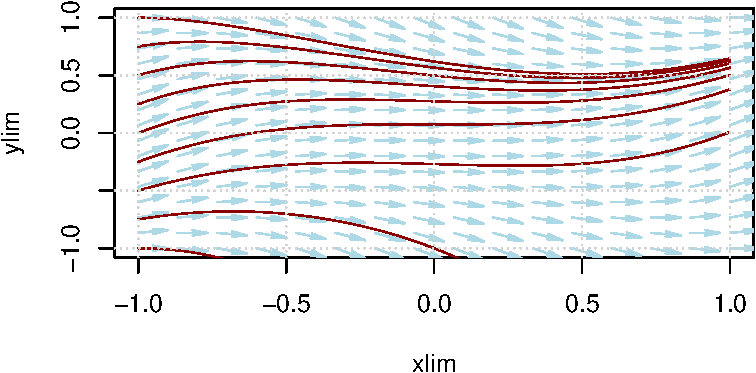
\includegraphics{index_files/figure-pdf/unnamed-chunk-5-1.pdf}




\end{document}
